
\subsection{dot product}
\begin{derv*} Geometrically speaking the dot product shows how much two vectors are covarying in the same
direction. Given two vectors $v$ and $w$,
\begin{equation}
   v \cdot w = ||w|| \big(||v||\cos \theta \big).
\end{equation}
When written as 
\begin{equation} \label{eq:vdotwn} %normalized w
   v \cdot \frac{w}{||w||} = ||v|||\cos \theta,
\end{equation}
this shows how much $v$ is projected in the direction of $w$. This demonstrates if the magitude of
both vectors are fixed, then the closer they are oriented, the more $v$ is projected onto $w$. The
greatest magnitude occurs when they overlap in the same direction $v \cdot w = ||v||||w||$. The
product is subject to the size of $v$ and $w$, so to compare how much one varies in the direction of
the other will need normalization as \eqref{eq:vdotwn}.
\begin{figure}[H]
   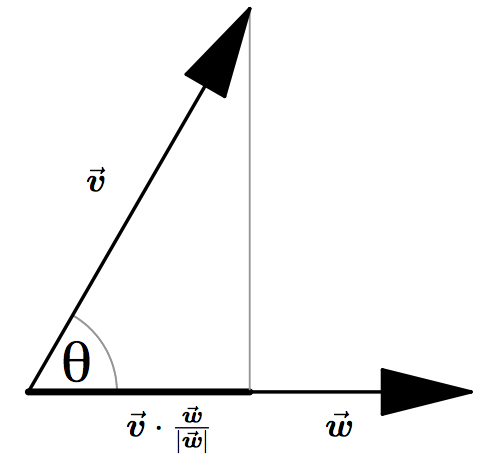
\includegraphics[width=0.3\textwidth, height=0.3\textwidth]{vdotw.png}
   \caption{\label{fig:vdotw}
      Dot product is a projection without normalization.}
\end{figure}
\end{derv*}

\subsection{Visualize linear transformation of a function as a matrix} 
Suppose $T: V \in \mathcal{R}^n \rightarrow W \in \mathcal{R}^m$, hence $T(x_1,\ldots,x_n) =
(b_1,\ldots,b_m)$, where $x_j$ and $b_i$ are the coordinate associated to the respective basis, and
$M(T,(e_1,\ldots,e_n),(f_1,\ldots,f_m))$. \\ 
What does a matrix do?  
\begin{enumerate} 
    \item Each domain basis vector is tranformed to the codomain as a vector 
        \begin{equation} 
            Te_j = a_{11}f_1 + \cdots + a_{m1}f_m = 
            \begin{pmatrix} a_{11} \\ \vdots \\ a_{m1} \end{pmatrix}, 
        \end{equation} 
        i.e.\, each basis vector $e_j \in V$ is mapped to the space spanned by $f_i$'s, recorded by the
        unique values of the $j$th column vector of $M(T)$.  
    \item $Tv = T(x_{1}e_{1} + \cdots + x_{n}e_{n}) = x_{1}Te_{1} + \cdots + x_{n}Te_{n} = x_{1}
        \begin{pmatrix} a_{11} \\ \vdots \\ a_{m1} \end{pmatrix} +
        \ldots x_{n} {\begin{pmatrix} a_{1n} \\ \vdots \\ a_{mn}\end{pmatrix}} =
        \begin{pmatrix} b_{1} \\ \ldots \\ b_{m} \end{pmatrix}$, where $b_{i} = a_{ij}
        x_{j}$ or $b_{i}f_{i} = \sum_{j} a_{ij} x_{j}f_{i}$. 
        This helps visualize that each basis vector $e_j$ is first mapped to the space of $W$ recorded by a
        column vector and individually stretched by $x_j$'s and combined to form a vector in $W$.  
\end{enumerate}

\subsection{What is linear algebra?} 
    \begin{itemize} 
        \item Solving system of equations $Ax = b$?  If treated the equations as hyperplanes $a_i^{T}x = b_i$, then we are finding the intersection points.  
        \item Finding the unique vector $x$ that gets mapped to $b$ by the linear function $A$?  
        \begin{itemize} 
            \item If treated $A$ as a linear operator on the same basis, then we are 
                  finding $x$ that gets mapped by $A$ to $b$ in the same domain.  
            \item If treated $A$ transforming between different basis for 
                  $x=x_{1}e_{1} + \cdots + x_{n}e_{n}$ and $b = b_{1}f_{1} + \cdots + b_{m}f_{m}$, 
                  then we are finding $x$ in the domain that gets mapped by $A$ to $b$ in the codomain.  
       \end{itemize} 
    \end{itemize}

\subsection{Invertible function} Definition: If $AB = I$, then $B$ is the inverse function of $A$.  \\
    \begin{exmp}
        Prove that if $ABw_{j} = w_{j}$, then $a_{j \cdot}^{T}b_{\cdot j} = 1$ and $AB$ is an identity matrix. \\ 
        Proof: \\ 
        $ABw_{j} = A(\sum_i b_{ij}v_i) = \sum_{i} b_{ij}(Av_{i}) = \sum_{i} b_{ij}(\sum_k a_{ki} w_{k}) = \sum_i\sum_{k} b_{ij} a_{ki} w_{k} $.  
        If $ABw_{j} = w_{j}$, then $\sum_{i}\sum_{k} b_{ij} a_{ki}w_{k} = w_{j}$ if and only if  $\sum_{i} a_{ki}b_{ij} \delta_{kj} = a_{j\cdot}^{T}b_{\cdot j} = 1$.  
        $AB$ is an identity matrix. 
    \end{exmp}

\subsection{How to solve eigenvalues of a matrix without determinant}
    Use Gauss elimination to the last pivot and find the eigenvalues.


\subsection{Karhunen Luoeve Expansion} 
    Q1: What is the expansion done on? The random variables at each random variable index? Or the entire random process/field expanded? \\ 
    A1: Expanded as a random process, not individual random variables expanded (as the PCE does). \\ 
    Q2: Where do you get the eigenvalues and eigenfunctions? \\ 
    A2: In terms of continuous random process/fields, the integral (linear operator) of 
        the continuous covariance function over a invariant function gives the eigenfunction and the corresponding eigenvalue.  
        In a discrate random process, the integral on the covariance matrix (PSD) $C$ is 
        just the inner product of the convariance vector of a random variable and the eigenvector. \\ 
    Q3: What ``variance'' is the eigenvalues associate with? \\ 
    A3: The projection of a single realization of a random process on a eigenfunction gives a random coefficient.  
        The variance of the collection of all the realizations of the random coefficient shows how much the random process varies in the direction of the eigenfunction.  
        This variance equals to the eigenvalue!
    

\subsubsection{\bf Mercer's Thm:}  Given a continuous symmetric positive semidemfinite (PSD) kernel $K$ on the random process/field $X_s$, the kernel can be expanded as 
    \begin{equation} 
        K(x,s) = \sum_i \lambda_i e_i(x) e_i(s).  
    \end{equation}

    {\bf Proof}: \\ 
    Given a covariance kernel (PSD) $K(x,s) = \Exp[X_{x}X_{s}]$, 
    and $K: [a \ b] \times [a \ b] \rightarrow \mathcal{R}$, 
    where $x$ and $s$ is the continuous index of the random variables.  
    Associated to $K$ is a linear operator $T_K$ on functions $\phi$ (covariance matrix operating on vectors is the discrete case) defined as 
    \begin{equation} 
        [T_K \phi](x) = \int_{[a \ b]} K(x,s) \phi(s) ds.  
    \end{equation} 
    To visualize this function, if we fix $x$ at a point, then the $K(x,s)$ and $\phi(s)$ are both functionals over the domain $s$.  
    The integration (inner product in discrete $s$) acts as how much $K(x,s)$ is related to the mode $\phi(s)$.  
    By testing over all $x$ (all rows), one could possibly find a mode (eigenvector) that is perfectly stretched in the mode direction.  
    Which is all rows of $K(x,s)$ relate to (by inner product) the mode with a single factor (eigenvalue).  
    Therefore, if there is a basis $\phi(s)$ that best represents (captures the variance) the covarying feature of the random process in $s$.  
    Then we could build a diagonal covariance matrix with this basis.  
    {\bf Since $T_K$ is a linear operator, we can talk about the eigenfunctions and eigenvalues of $T_K$}.  
    Therefore, the eigenfunctions associated to the linear operator has the representation 
    \begin{equation} 
        [T_K e_k](x) = \int_{[a \ b]} K(x,s) e_k(s) ds = \lambda_k e_k, 
    \end{equation} 
    where $e_k$'s are orthonormal wrt the linear operator $\int_{[a \ b]} e_k e_j ds = \delta_{kj}$.  
    By plugging in $K(x,s) = \sum_i \lambda_i e_i(x) e_i(s)$ to the lhs equation 
    \begin{equation} 
        \int_{[a \ b]} \sum_i \lambda_i e_i(x) e_i(s) e_k(s) ds = \lambda_i e_k(x), 
    \end{equation} 
    where orthogonality is used.  
    This shows that in fact $K(x,s) = \sum_i \lambda_i e_i(x) e_i(s)$. 
    $\blacksquare$ \\ 
    If $X$ is a discrete random process/field, then 
    $[T_K e_k](x_i) = \sum_j K(x_i,s_j) e_k(s_j) = \lambda_k e_k(x_i)$ 
    is the inner product of the covariance vector of the $i$th random variable
    ($i$th row of the convariance matrix) and the eigenvector $e_k( \vec{s})$.  
    From spectral theory of a PSD matrix, the covariance matrix (PSD) also yields an 
    eigen-decomposition $K = V\Lambda V^T$, with $K_{ij} = \Exp[X_{x_i}X_{s_j}] = \sum_k \lambda_k e_k(x_i) e_k(s_j) $. \\ 
    (Notice: the integral operator is not the expectation operator, so the expectation is only in the covariance kernel, but not shown explicitly) \\
    
\subsubsection{\bf Karhunen Luoeve's Thm:} 
    Prove that a zero-mean square integrable stochastic process $X_t$ with continuous covariance function can be represented as 
    \begin{equation} 
        X_t = \sum_{k=1}^\infty Z_k e_k(t) 
    \end{equation} 
    where $Z_k = \int_a^b X_t e_k(t) dt$.  
    Furthermore, prove $\Exp[Z_{k}] = 0$ and $\Exp[Z_{k}Z_{j}] = \delta_{kj}\lambda_{k}$ 
    (the variance of $Z_{k}$, how much $X_{t}$ varies in the direction of $e_{k}$ in the mean, is just the eigenvalue of the covariance function). \\ 
    
    {\bf Proof}: \\ 
    From the Mercer's Thm, $K(x,s) = \sum_{i} \lambda_{i} e_{i}(x) e_{i}(s)$.  
    By projecting $X_t$ onto the eigenfunctions obtained from $K$, $Z_k = \int_a^b X_t e_k(t) dt$, and we can form $X_t = \sum_{k=1}^\infty Z_k e_k(t)$.  
    Thus, 
    \begin{equation} 
        \Exp[Z_k] = \Exp[\int_a^b X_t e_k(t) dt] = \int_a^b \Exp[X_t] e_k(t)dt = 0, 
    \end{equation} 
    and 
    \begin{equation} 
        \Exp[Z_{i}Z_{j}] = \delta_{ij} \lambda_{i} \ (\text{This is a simple proof!}).  
    \end{equation}

    {\bf Conclusion}: \\ Eigenvalues represent the variance of the random process in the direction of the 
    eigenvectors! This is why using the eigenvectors from decomposing the symmetric PSD covariance function makes sense!

\subsection{Lyapunov Exponent} 
    Given a linear dynamic system with known linear parameters a,b,c and d, 
    \begin{equation} 
        \frac{d}{dt} 
        \begin{pmatrix} x_1 \\ x_2 \end{pmatrix} = 
        \begin{pmatrix} a & b \\ c & d \end{pmatrix} 
        \begin{pmatrix} x_1 \\ x_2 \end{pmatrix} = A 
        \begin{pmatrix} x_1 \\ x_2 \end{pmatrix}.  
    \end{equation} 
    The eigenvalues and eigenvectors of $A$ can be obtained fairly easily, with eigenvalues being either complex or real.  
    The orthonormal eigenvectors $v_1$ and $v_2$ are treated as the basis and the state $x$ 
    can be expanded as $x = c_1v_1 + c_2v_2$ (just as EOFs spanning the space of the multivariate space).  
    Therefore the system becomes 
    \begin{equation} 
        \frac{d}{dt} \begin{pmatrix} c_1 \\ c_2 \end{pmatrix} = \begin{pmatrix} \lambda_1 & 0 \\ 0 & \lambda_2 \end{pmatrix} \begin{pmatrix} c_1 \\ c_2 \end{pmatrix}. 
    \end{equation} 
    This gives the evolution equation of the coefficients by using the invariant eigenvectors.  
    The coefficients has the general solution form $c_i(t) = c_i(0)e^{\lambda_i t}$, where the stability is determined by the real or complex of the $\lambda_i$'s.  
    The coefficients determines how much the states are projected onto the eigenvectors at any time.


\subsection{Self-Adjoint and Normal Operator} 
    linear functional: $\phi(v)= <v,u>$, $u$ is a ``unique vector'' in $V$ for this
    functional $\mathcal{R}^{n} \rightarrow \mathcal{R}$. \\
%   polynomial is a vector in $P_n(\mathcal{R}), not a functional, one could
%   define a functional for polynomial vectors (with orthonormal basis over the
%   inner product) \phi(p)=<p,q>, with inner product $<\cdot,\cdot>=\int_0^1 pq
%   dx$.  
    Define adjoint function from the linear functional: $\phi(v)= < Tv, w>$, one
    can find the unique vector of this linear functional to be $T^*w \in V$
    satisfying $< Tv, w> = <v, T^*w>$, $T^*$ is the adjoint of $T$. \\ 
%   \phi(v) finds the cov of v, transform by T into W, and w.  The cov is the same
%   as w, transform by $T^*$ into V, and v.  
            
    {\emph{\bf Example:} \\ Suppose $T:\mathcal{R}^3 \rightarrow \mathcal{R}^2$ and
    $T(x_1,x_2,x_3)= (x_1+x_2,x_3)$.  The adjoint $T^*$ is $T^*(y_1,y_2)$,
    therefore $< T(x_1,x_2,x_3),(y_1,y_2)> = x_1y_1+x_2y_1+x_3y_2 =
    <(x_1,x_2,x_3),T^*(y_1,y_2)> \Rightarrow T^*(y_1,y_2)=(y_1,y_1,y_2)$. \\ }

\subsection{Kernel PCA} 
    Given a $d$-dim random variable $\bm x$ with $N$ random samples, the general
    PCE operates on zero-centered data 
    \begin{equation} 
        \Exp (\bm x)= \frac{1}{N} \sum\limits_i^N \bm x_i = \bm{0}   
    \end{equation}

    with covariance matrix \begin{equation} \Exp (\bm x^2)= \frac{1}{N}
    \sum\limits_i^N \bm x_i \bm x_i^T \end{equation} which is a matrix of the
    average of a set of outer product matrices, or can be seen as a matrix with
    entries of the averaged inner product of a single dimension r.\ v.\ with $N$
    samples.



\subsection{Generalized Eigenvalue Decomposition (2$\nnd$ kind)} 
\subsubsection{Definition} Given a pair of Hermitian matrices $(A, B) \in \mathcal{S}^n$, 
    the generalized eigenvalue is the roots of $p(\lambda)= \det(A-\lambda B)=0$ satisfying the relationship 
    \begin{equation} 
       Av= \lambda Bv.  
    \end{equation} 
    Notice the generalized eigenvectors need not be orthogonal!  
    The standard eigenvalue decomposition is just ordering $\lambda_i$ in nonincreasing order, and denote the maximum generalized eigenvalue by $\lambda_{\max}(A,B)$.  

\subsubsection{Special case} If $B \in \mathcal{S}_{++}^n$, 
    we know that positive definite matrix has positive definite square root 
    ($B^{\onehalf}={(B^{\onehalf})}^{*}$), $B= B^{\onehalf}{(B^{\onehalf})}^{*}= B^{\onehalf}B^{\onehalf}$.  
    Therefore 
    \begin{equation} 
        AV= B^{\onehalf}B^{\onehalf}V \Lambda \Rightarrow B^{-\onehalf}AB^{-\onehalf}B^{\onehalf}V= B^{\onehalf}V \Lambda \Rightarrow B^{-\onehalf}AB^{-\onehalf}V'=V'\Lambda, 
    \end{equation} 
    implies the generalized eigenvalues of $(A,B)$ are the same as the eigenvalues of $B^{-\onehalf}AB^{-\onehalf}$ when $B \in \mathcal{S}_{++}^n$.  
    Since $V' \Lambda V'^T$ is the eigenvalue decomposition of $B^{-\onehalf}AB^{-\onehalf}$, the \emph{generalized eigenvalue decomposition} 
    \begin{equation} 
        B^{-\onehalf}AB^{-\onehalf} = V'\Lambda V'^T \Rightarrow A = 
        B^{\onehalf}V' \Lambda V'^{T}B^{\onehalf} \Rightarrow A = Q \Lambda Q^{T} \hspace{1cm} B = 
        B^{\onehalf}B^{\onehalf}= B^{\onehalf}V'V'^{-1}B^{\onehalf}= QQ^T.  
    \end{equation}


\section{Chapter 8 Operators on Complex Vector Space}

    This chapter is aimed to find the space spanned by the generalized eigenvectors of an operator (not
    all operators have enough eigenvectors). \\

    \noindent {\bf Definition of Generalized Eigenvectors:} \\
    $v$ is the generalized eigenvector of $T$ corresponding to $\lambda$ if $v \in \nullt(T-\lambda
    I)^j$. \\

    \noindent {\bf Properties of generalized eigenvectors} 
    \begin{itemize}
        \item Inclusion : $\{0\} = \nullt(T-\lambda)^{0} \subset \nullt(T-\lambda)^{1} \subset \cdots
            \subset \nullt(T-\lambda)^{k} \subset \cdots$
        \item Saturation : $\nullt(T-\lambda)^{0} \subset \cdots \subset
            \nullt(T-\lambda)^{m} = \nullt(T-\lambda)^{m+1} = \cdots$
        \item Maximization : $\nullt(T-\lambda)^{\dims V} = \nullt(T-\lambda)^{\dims V+1} = \cdots$
    \end{itemize}

    \noindent {\bf Remarks : Space of the generalized eigenvectors is $\nullt(T-\lambda)^{\dims V}$ !!} \\

    \noindent {\bf Defining a Nilpotent operator using generalized eigenvectors } 
    \begin{itemize}
        \item Operators going to zero at some power, and the entire vector space is the generalized
            eigenvector space with respect to the zero eigenvalue.
    \end{itemize}

    \noindent {\bf Remarks : The power for a nilpotent operator must be contained by $\dims V$, $N^{\dims
    V} = 0$.}




